%
% File emnlp2016.tex
%

\documentclass[11pt,letterpaper]{article}
\usepackage{emnlp2016}
\usepackage{times}
\usepackage{latexsym}
\usepackage{url}
\usepackage{graphicx}
\usepackage{caption}% <-- added
\usepackage{tabularx,booktabs}
\newcolumntype{C}{>{\centering\arraybackslash\hsize=.5\hsize}X} % centered version of "X" type
\setlength{\extrarowheight}{1pt}
\usepackage{makecell}


\renewcommand\theadalign{bc}
%\renewcommand\theadfont{\bfseries}
\renewcommand\theadgape{\Gape[4pt]}
\renewcommand\cellgape{\Gape[4pt]}

% Uncomment this line for the final submission:
\emnlpfinalcopy


% To expand the titlebox for more authors, uncomment
% below and set accordingly.
% \addtolength\titlebox{.5in}    

\newcommand\BibTeX{B{\sc ib}\TeX}


\title{Part-of-Speech Tagging with LSTMs}

% Author information can be set in various styles:
% For several authors from the same institution:
% \author{Author 1 \and ... \and Author n \\
%         Address line \\ ... \\ Address line}
% if the names do not fit well on one line use
%         Author 1 \\ {\bf Author 2} \\ ... \\ {\bf Author n} \\
% For authors from different institutions:
% \author{Author 1 \\ Address line \\  ... \\ Address line
%         \And  ... \And
%         Author n \\ Address line \\ ... \\ Address line}
% To start a seperate ``row'' of authors use \AND, as in
% \author{Author 1 \\ Address line \\  ... \\ Address line
%         \AND
%         Author 2 \\ Address line \\ ... \\ Address line \And
%         Author 3 \\ Address line \\ ... \\ Address line}
% If the title and author information does not fit in the area allocated,
% place \setlength\titlebox{<new height>} right after
% at the top, where <new height> can be something larger than 2.25in
\author{Zeyuan Hu \\
  Computer Science Department \\
  University of Texas at Austin \\
  Austin, Texas \\
  {\tt iamzeyuanhu@utexas.edu} \\
}

\date{}

\begin{document}

\maketitle

\begin{abstract}
	We build a Bidirectional Long Short Term Memory networks (BiLSTMs) and apply it 
	to Part-Of-Speech (POS) tagging using data from the Penn Treebank \cite{Marcus:1994}.
	We incoporate orthographic features (e.g., capitalization, suffix, prefix) into the model
	and improve the baseline model overall accuracy by 1\% and OOV accuracy by 23.1\% on the validation set, 
	and 0.8\% overall accuracy and 24.4\% OOV accuracy on the test set.
\end{abstract}

\section{Introduction}

Parts-of-Speech (POS) tagging is a task that assigns a tag to each word in a given sentence.
Tag may include: noun, verb, pronoun, preposition, adverb, and so on. 
POS tagging is an important task in NLP because knowing the tags of words can
give us the information about likely neighbouring words 
and the syntactic structure of the sentence,
which will be useful for Syntactic Parsing, Named Entity Recognition, and other 
information extraction tasks \cite[Chapter~10]{Jurafsky:2017}. However, since the amount
of tags and sentences can be large, manually tagging each words in a sentence
can be extremely time-consuming. Thus, we want to invoke some statistical model
to automatically generate the tags for us. In this report, we employ
the Bidirectional Long Short Term Memory networks (BiLSTMs) model.

Bidirectional Long Short Term Memory networks (BiLSTMs) model is one
kind of Long Short Term Memory network (LSTM) models with architecture shown in
Figure \ref{fig:1} \cite{cs224d}. $x$ represents a token (word) as a vector;
$y$ represents the output POS tag; and $h$ represents the memory, which is
computed from the past memory and current word \cite{colah}. The motivation
for us to use BiLSTMs model is that POS tagging is a classification problem 
(i.e., we classify each word into one of the tag category) and for classification
on a given word, we want to incorporate information from both the preceding
words (i.e., forward direction in BiLSTMs) and the words following it
(i.e., backward direction in BiLSTMs).

\begin{figure}
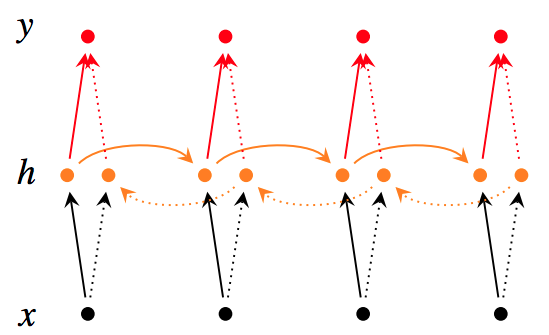
\includegraphics[scale=0.35]{bilstm-architecture.png}
\caption{BiLSTMs Architecture}
\label{fig:1}
\end{figure}

\section{Orthographic Features}

Baseline uses the BiLSTMs model with the {\fontfamily{qcr}\selectfont <\texttt{word\_ID}, \texttt{pos\_tag}>}
pair. In other words, words are represented by its \texttt{word\_ID} in the vocabulary and fed into the
model. In this report, besides word ID, we use the following orthographic features from each word to improve the model 
performance:

\begin{itemize}
\item Capitalization
\item Contains common English suffix \cite{suffix} \footnote{We use 31 prefixes and 23 suffixes.}
\item Contains common English prefix \cite{suffix}
\item Contains hyphen
\item Starts with a number
\end{itemize}

%The prefixes we use are \texttt{anti-, de-, dis-, en-, em-, fore-, in-, im-, il-, ir-, inter-,
%mid-, mis-, non-, over-, pre-, re-, semi-, sub-, super-, trans-, un-, under-} and the suffixes
%we use are \texttt{-able, -ible, -al, -ial, -ed, -en, -er, -er, -est, -ful, -ic, -ing, -ion, -tion,
%-ation, -ition, -ity, -ty, -ive, -ative, -itive, -less, -ly, -ment, -ness, -ous, -eous, -ious, -s, -es, -y} 
%\cite{suffix} \footnote{We use 31 prefixes and 23 suffixes.}.

The intuition for using these orthographic features is that orthographic features may be good indicators for building
the connection between words and POS tags. For example, capitalization may be a strong indicator for 
\texttt{PRP} (e.g., \emph{I}) or \texttt{NNP} (e.g., \emph{China}). Similarly, prefix (e.g., \emph{anti-}) and suffix (e.g., \emph{-ly}) 
are good indicators for \texttt{NN} (e.g., \emph{ant-government}) and \texttt{RB} (e.g., \emph{lovely}) respectively.

\section{Implementation}

Orthographic features are represented by its ID in the corresponding ``feature vocabulary" like
we do with word ID feature. For example, capitalization is a binary feature: whether a word contains
capitalization: $1$ means ``yes" and $0$ means ``no". Thus, for capitalization feature, the ``feature
vocabulary" has size of $2$. We construct such ``feature vocabulary" for each feature during the preprocessing
step.

We use two ways to incoporate the orthographic features into BiLSTMs model: at the input and at the output.
Figure \ref{fig:2} shows an implementation view of BiLSTMs when we incoporate the orthographic
features at the input. At the input, orthographic features are concatenated with the original
word ID feature. Each column (one is colored in green) in Figure \ref{fig:2} is a vector representation of a word
(``was" in this case). The vector is constructed by concatenating the vector representation of each feature.
The dimension for word ID feature is $\texttt{embedding dimension} \times 1$. The rest features (i.e., all
orthographic features) will have their dimensions determined the way we construct them. We use three ways
to construct the orthographic feature vectors: \emph{embedding}, \emph{one\_hot}, and \emph{int}. \emph{embedding}
constructs the orthographic features in exactly the same way as the word ID feature: using embedding.
The only difference is that we embedd the orthographic features into dimension $\texttt{orthographic\_embedding\_dim} \times 1$
with $\texttt{orthographic\_embedding\_dim}$ set to 10 by default. \emph{one\_hot} option is similar to \emph{embedding}
but we use the size of each ``feature vocabulary" to determine the one-hot vector dimension. The advantage of
doing so over the \emph{embedding} is that each orthographic feature's one-hot vector may have different length. Since the
size of ``feature vocabulary" is very small (i.e., the largest size is 31), we do not need to worry about the computation
inefficency brought by one-hot vector. The last way is \emph{int}, which directly feed the feature ID as part of word vector
representation into BiLSTMs.

When we concatenate the orthographic features into the BiLSTMs at the output, we use the same ways to construct
our orthographic feature vector representations. The only difference is that we concatenate our orthographic features
with the outputs from BiLSTMs. The outputs of BiLSTMs is connected with a fully connected layer so that we can know
that which POS tag has the highest probability for the corresponding word. The fully connected layer is needed because
we need to map the output dimension from BiLSTMs into the dimension that is well-aligned with the number of POS tags.
By concatenating orthographic features at the output, we increase the dimension of the output vector that is to be fed
into the fully connected layer.

\begin{figure}
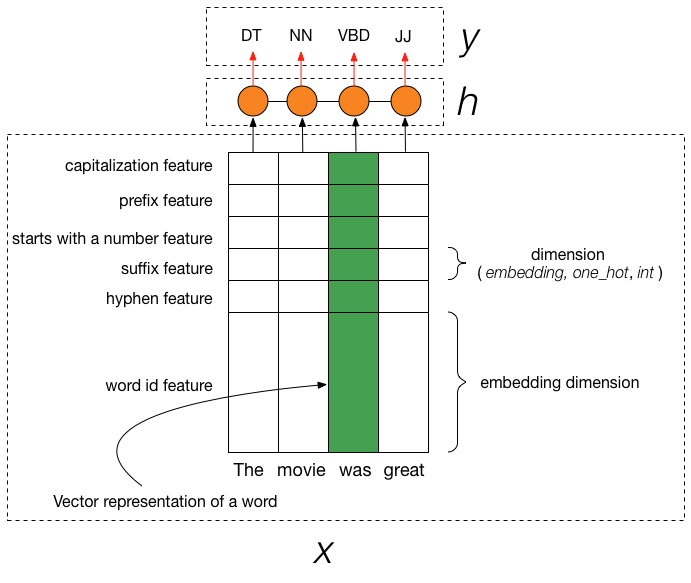
\includegraphics[scale=0.35]{LSTM.png}
\caption{BiLSTMs Implementation when Adding Orthographic Features at the Input}
\label{fig:2}
\end{figure}

\section{Experiments and Analysis}
\label{ssec:layout}

We perform six experiments: two place to concate orthographic features in combination
with three ways to construct feature vector representations. The hyperparameters for
the experiments are shown in Table \ref{tab:freq}.  All the experiements are performed on
a machine that has 4 Intel(R) Core(TM) i5-6200U CPU @ 2.30GHz processors and 4GB of memory.
Experiment results are shown in Table \ref{valid} and Table \ref{test}.

\begin{table}
\captionsetup{size=footnotesize}
%\setlength\tabcolsep{0pt} % let LaTeX compute intercolumn whitespace
\footnotesize\centering
%This table provides the frequencies.

\smallskip 
\begin{tabular*}{\columnwidth}{@{\extracolsep{\fill}}lc}
\toprule
  Description  & Values  \\
\midrule
 batch size & 128      \\
 number of epochs & 6 \\
 embedding size for word ID & 300        \\
 embedding size for orthographic features & 10        \\
 optimizer learning rate & 0.0005 \\
 optimizer & Adam \\
\bottomrule
\end{tabular*}
\caption{BiLSTMs Configuration} \label{tab:freq}
\end{table}

\begin{table}[]
\centering
\scalebox{1.1}{
\begin{tabular}{|l|l|l|l|}
\hline
Validation & \multicolumn{3}{l|}{BASELINE}           \\ \hline
           & Accuracy & \thead{OOV \\ Accuracy} & \thead{Training \\ Time} \\ \hline
embedding  & 95.6\%   & 57.1 \%       & 860s          \\ \hline
one\_hot   & 95.6\%   & 57.1 \%       & 860s          \\ \hline
int        & 95.6\%   & 57.1 \%       & 860s          \\ \hline
           & \multicolumn{3}{l|}{INPUT}              \\ \hline
           & Accuracy & \thead{OOV \\ Accuracy} & \thead{Training \\ Time} \\ \hline
embedding  & 96.5\%   & 78.3\%       & 927s          \\ \hline
one\_hot   & \textbf{96.6\%}   & \textbf{80.2\%}       & 911s          \\ \hline
int        & 96.1\%   & 66.7\%       & \textbf{859s}          \\ \hline
           & \multicolumn{3}{l|}{OUTPUT}             \\ \hline
           & Accuracy & \thead{OOV \\ Accuracy} & \thead{Training \\ Time} \\ \hline
embedding  & 96.1\%   & 70.5\%       & 878s          \\ \hline
one\_hot   & 95.6\%   & 57.2\%       & 885s          \\ \hline
int        & 95.5\%   & 56.6\%       & 878s          \\ \hline
\end{tabular}}
\caption{Model Performance on Validation Set}
\label{valid}
\end{table}

\begin{table}[]
\centering
\scalebox{1.1}{
\begin{tabular}{|l|l|l|}
\hline
Test      & \multicolumn{2}{l|}{BASELINE} \\ \hline
          & Accuracy & \thead{OOV \\ Accuracy} \\ \hline
embedding & 95.8\%   & 55.4\%       \\ \hline
one\_hot  & 95.8\%   & 55.4\%       \\ \hline
int       & 95.8\%   & 55.4\%       \\ \hline
          & \multicolumn{2}{l|}{INPUT}  \\ \hline
          & Accuracy & \thead{OOV \\ Accuracy} \\ \hline
embedding & \textbf{96.6\%}   & \textbf{78.8\%}       \\ \hline
one\_hot  & \textbf{96.6\%}   & 77.7\%       \\ \hline
int       & 96.1\%   & 66.3\%       \\ \hline
          & \multicolumn{2}{l|}{OUTPUT}   \\ \hline
          & Accuracy & \thead{OOV \\ Accuracy} \\ \hline
embedding & 96.2\%   & 70.4\%       \\ \hline
one\_hot  & 95.6\%   & 57.2\%       \\ \hline
int       & 95.7\%   & 54.2\%       \\ \hline
\end{tabular}}
\caption{Model Performance on Test Set}
\label{test}
\end{table}

%%https://tex.stackexchange.com/questions/2441/how-to-add-a-forced-line-break-inside-a-table-cell
%%https://tex.stackexchange.com/questions/10863/is-there-a-way-to-slightly-shrink-a-table-including-font-size-to-fit-within-th
%%https://tex.stackexchange.com/questions/89462/page-wide-table-in-two-column-mode
%\begin{table*}[t]
%\centering
%\caption{My caption}
%\label{my-label}
%\scalebox{0.8}{
%\begin{tabular}{|l|l|l|l|l|l|l|l|l|l|}
%\hline
%Validation & \multicolumn{3}{l|}{BASELINE}           & \multicolumn{3}{l|}{INPUT}              & \multicolumn{3}{l|}{OUTPUT}             \\ \hline
%           & Accuracy & \thead{OOV \\ Accuracy} & \thead{Training \\ Time} & Accuracy & \thead{OOV \\ Accuracy} & \thead{Training \\ Time} & Accuracy & \thead{OOV \\ Accuracy} & \thead{Training \\ Time} \\ \hline
%embedding  & 95.6\%   & 57.1\%       & 860s          & \textbf{96.5\%}   & 78.3\%       & 927s          & 96.1\%   & 70.5\%       & 878s          \\ \hline
%one\_hot   & 95.6\%   & 57.1\%       & 860s          & 96.6\%   & 80.2\%       & 911s          & 95.6\%   & 57.2\%       & 885s          \\ \hline
%int        & 95.6\%   & 57.1\%       & 860s          & 96.1\%   & 66.7\%       & 859s          & 95.5\%   & 56.6\%       & 878s          \\ \hline
%\end{tabular}}
%\end{table*}

From the results, we can see that adding the orthographic features increases the BiLSTMs performance on
both the overall accuracy and the OOV accuracy on both validation set and test set. For the validation set,
adding the orthographic features as one-hot vectors at the input improves the baseline performance by 1\%. At the same time,
there is a large jump on OOV accuracy, which raises from 57.1\% to 80.2\% (i.e., 23.1\% increase). The tradeoff
for more accurate model is the longer training time. To train orthographic-enhanced BiLSTMs with \emph{one\_hot}
takes 51 more seconds. Surprisingly, if we directly add feature ID as the input, the running time is actually
similar to baseline model. The reason behind this is that adding feature ID as the input does not increase computational
complexity (i.e., does not involve significant matrix multiplication and transformation).

On the test set, the story is similar with \emph{embedding} and \emph{one\_hot} at the input leading the chart. From these
two tables, we can see that adding the orthographic features at the input outperforms adding
the orthographic features at output (i.e., classification layer). One possible reason is that adding the orthographic features
at the input provides BiLSTMs a chance to learn the weights of features according to the ground truth. However, if we
directly add the orthographic features at the classification layer, there is no chance for the model to fine tune the weights.
In addition, adding the orthographic features at the input enriches the information encoded in the vector representation of a word.
By incorporating more characteristic information about a word in the vector representation, we can better learn the connection
between word and POS tag. Adding orthographic features at the output, however, is not all bad. From the experiment results we can see
that adding orthographic feature at the classification layer generally requires less training time compared with at the input.
This is because computation at the memory units of BiLSTMs is much more complex than the computation at the fully connected output layer.
Thus, sending larger vector to the memory units (i.e., adding orthographic features at the input) takes more time to compute than sneding larger
vector to the classification layer (i.e., adding orthographic features at the output). 

%Overall, how does adding orthographic features affect the accuracy (both overall and OOV) and runtime of the BiLSTM and why?
%How does changing the approach to adding these features (input vs. classification layer) affect the accuracy (both overall and OOV) and runtime of the BiLSTM and why?

\section{Conclusion and Future Work}
\label{ssec:first}

In this report, we use orthographic features to improve the BiLSTMs model overall
accuracy by 1\% and OOV accuracy by 23.1\% on the validation set, and 0.8\% overall
accuracy and 24.4\% OOV accuracy on the test set. As the following, we show that orthographic
features can indeed improve the model performance. In the future, we may want to experiment
with different languages to see if our conclusion still holds.
\bibliography{emnlp2016}
\bibliographystyle{emnlp2016}

\end{document}
